\section{Comunicazione}\label{capitolo5}
La comunicazione tra processi è il cuore di tutti i sistemi distribuiti, infatti, non ha senso studiare i sistemi distribuiti senza esaminare come i processi su posti macchine diverse si scambiano le informazioni. La comunicazione nei sistemi distribuiti si basa sempre sullo scambio dei messaggi a basso livello come fornito dalla rete sottostante, anche se ciò rende la realizzazione del sistema distribuito molto complicata.\\
In questo capitolo analizzeremo prima di tutto le regole che i diversi processi devono rispettare per comunicare tra loro, queste regole sono conosciute anche come protocolli e solitamente vengono strutturati a livelli.\\
Analizzeremo in seguito tre modelli di comunicazione molto diffusi, le chiamate a procedure remote (RPC, \emph{remote procedure call}), i middleware orientati agli oggetti (MOM, \emph{message-oriented middleware}) e gli \emph{streaming} di dati. Ed infine analizzeremo il problema dell'invio di dati a destinatari multipli, ovvero, il \emph{multicast}.\\
\subsection{Il modello OSI}
A causa della mancanza di una memoria condivisa tutta la comunicazione nei sistemi distribuiti avviene mediante tramite l'invio e la ricezione di messaggi a basso livello. Quando un processo \emph{A} vuole comunicare con un processo $B$ prima di tutto costruisce un messaggio nel proprio spazio degli indirizzi e poi effettua una \emph{chiamata di sistema} che fa in modo che il SO si occupi dell'invio del messaggio attraverso la rete fino a raggiungere $B$. Anche se il principio è semplice esistono diversi ostacoli al completamente di questa operazione, prima di tutto $A$ e $B$ devono concordare sul significato dei bit inviati, esistono molti altri aspetti sui quali bisogna accordarsi, come il valore in volt usati per indicare un bit a 1, individuare l'ultimo bit del messaggio, bisogna inoltre capire se un messaggio è stato danneggiato o perso ecc.\\
Per poter trattare facilmente i numerosi aspetti di una comunicazione la \emph{international standards organization} (ISO) ha sviluppato un modello di riferimento che identifica i vari livelli di comunicazione coinvolti, gli assegna dei nomi standard e identifica le diverse funzionalità per ogni livello. Questo modello è chiamato \textbf{open system interconnection reference model} o più comunemente modello \textbf{ISO OSI} ed è illustrato in \figurename\,\ref{img:osi}
\begin{figure}[htb]
\centering
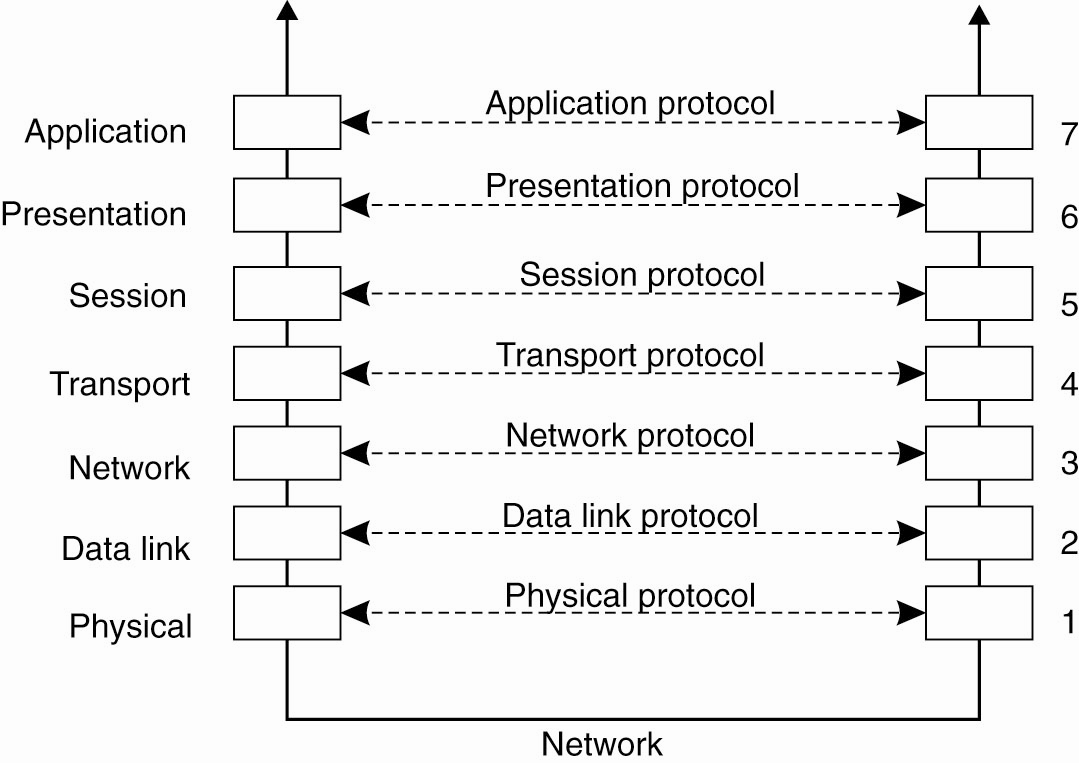
\includegraphics[scale=0.4]{img/osi.png}
\caption{Modello ISO OSI}\label{img:osi}
\end{figure}
Tuttavia è bene far presente che i protocolli sviluppati nel modello OSI non sono stati mai ampiamente utilizzati, tuttavia il modello sottostante si è rivelato particolarmente utile per comprendere le reti di computer.\\
Il modello OSI è progettato per consentire la comunicazione tra sistema aperti ovvero tra sistemi preparati per comunicare tramite regole standard che ne regolano il formato, i contenuti ed il significato di messaggi ricevuti ed inviati. Queste regole sono dette \textbf{protocolli} e devono essere concordate a priori per permettere la comunicazione tra gruppi di computer.\\
Esistono due grandi tipologie di protocolli, quelli \textbf{orientati alla connessione} nei quali mittente e destinatario stabiliscono esplicitamente una connessione prima di scambiarsi dei dati ed alla fine devono rilasciare tale connessione.
Con i protocolli \textbf{senza connessione} non è necessaria alcuna premessa, quando il messaggio è pronto il mittente invia il messaggio come nel caso di un invio di una lettera.\\
Nel modello OSI la comunicazione è suddivisa in sette livelli o \emph{layer}, ogni livello tratta uno specifico aspetto della comunicazione, in modo da suddividere il problema in parti gestibili ciascuna delle quali può essere trattata indipendentemente. Per realizzare questo meccanismo ogni livello fornisce un'interfaccia al livello superiore, la quale specifica un insieme di operazioni che il livello è pronto a fornire.\\
Quando un processo $A$ sulla macchina 1 vuole comunicare con un processo $B$ sulla macchina 2 costruisce un messaggio e lo passa al livello applicativo sulla sua macchina; tale livello potrebbe essere una procedura ad una libreria oppure implementato in qualche altro modo come ad esempio all'interno del sistema operativo. Il software a livello applicativo aggiunge un intestazione (\emph{header}) all'inizio del messaggio e passa tutto al livello di presentazione tramite l'interfaccia tra i livelli 6 e 7. A sua volta il livello di presentazione passa il messaggio al livello di sessione non prima di aver aggiunto il suo \emph{header} e così via. Alcuni livelli aggiungono oltre all'header anche un \emph{trailer} in chiusura al pacchetto come mostrato in \figurename\,\ref{img:header}.
\begin{figure}[htb]
\centering
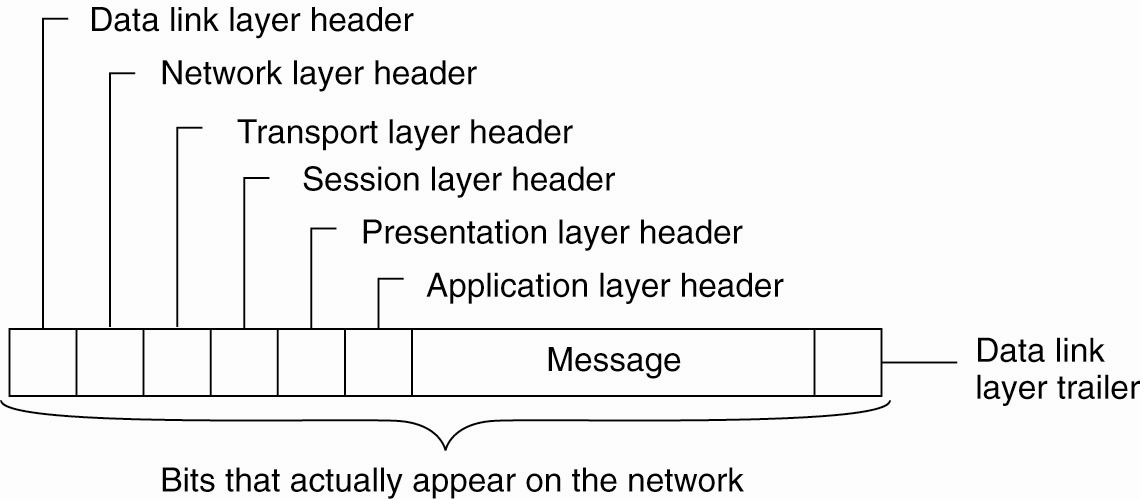
\includegraphics[scale=0.4]{img/header.png}
\caption{Elenco header e trailer di un messaggio che attraversa i vari layer}\label{img:header}
\end{figure}
Quando il messaggio raggiunge il fondo esso viene trasmesso dal livello fisico sul mezzo di trasmissione. Quando il messaggio raggiunge la macchina 2 viene passato verso l'alto e ogni livello stacca la sua intestazione e la esamina, infine il messaggio raggiunge il suo destinatario , ovvero il processo B il quale può rispondere utilizzando il percorso inverso.\\
Ogni livello ha il suo protocollo che può essere cambiato indipendentemente dagli altri ed è proprio questa indipendenza a rendere i protocolli a livelli interessanti.\\
L'insieme di protocolli usati in un particolare sistema è detto \textbf{suite di protocolli} o \textbf{stack di protocolli}.
\subsubsection{I layer}
Analizziamo ora i diversi layer che compongono il modello OSI, vedremo quali sono le loro funzionalità e dove possibile indicheremo quali protocolli sono attualmente utilizzati nell'ambito di internet.
Partiamo dai tre livelli più bassi della suite di protocolli, insieme questi tre livelli implementano le funzioni base di una rete di computer.\\
Il \emph{livello fisico} trasmette gli 0 e gli 1 sul canale fisico di comunicazione, elementi importanti per questo livello sono la quantità di volt che contraddistingue gli 0 e gli 1, il numero di bit al secondo, la possibilità di trasmettere in entrambe le direzioni, infine rivestono una notevole importanza la forma dei connettori (\emph{plug}) ed il numero di piedini (\emph{pin}). Il protocollo che identifica questo livello ha a che fare con la standardizzazione delle interfacce elettriche e meccaniche e di segnale; un esempio di questi standard è l'interfaccia RS-232-C per la comunicazione seriale.\\
Il livello \emph{data link} si occupa della rilevazione e della correzione degli errori di trasmissione. Per fare ciò il data link layer raggruppa i bit in unità chiamate \textbf{frame} e controlla che ogni frame sia ricevuto correttamente. Per eseguire questo compito il livello di collegamento dei dati applica un \emph{pattern} di bit all'inizio ed alla fine di ogni frame per delimitarli ed eseguire una \textbf{somma di controllo} (\emph{checksum}) sommando tramite algoritmi specifici i byte del frame ed inserisce tale somma nei campi all'inizio o alla fine del frame.
All'arrivo di un nuovo pacchetto il livello data link esegue la somma sui dati arrivati e la confronta con quella inviata insieme al pacchetto nel caso le due checksum coincidano il pacchetto è considerato corretto, in caso contrario il destinatario ne richiede la ritrasmissione grazie al numero di sequenza inserito nell'header del data link.\\
Il \emph{livello di rete} si occupa del \textbf{routing} dei pacchetti, ovvero, della scelta del percorso ottimale che permetta ad un pacchetto di andare da un mittente ad un destinatario.
Il problema si complica in quanto il percorso più breve non è sempre quello ottimo. Al momento il protocollo di rete più utilizzato è l'IP (\textbf{Internet Protocol}) senza connessione che è parte dei protocolli Internet. Un \textbf{pacchetto} IP può essere inviato senza alcun preparativo. Ogni pacchetto è instradato verso la sua destinazione indipendentemente da tutti gli altri.\\
Il \emph{livello di trasporto} costituisce l'ultima parte di quelli che possiamo definire \emph{stack del protocollo di rete di base} nel senso che implementa tutti i quei servizi non forniti dall'interfaccia del livello di rete ma necessari per l'implementazione di applicazioni di rete. In altre parole il livello di trasporto in un qualcosa di utilizzabile.\\
Uno dei compiti del livello di trasporto è quello di fornire una connessione affidabile anche se molte applicazioni gestiscono autonomamente la perdita di pacchetti.
Quando arriva un messaggio dal livello applicativo il livello di trasporto lo spezza in parti sufficientemente piccole per essere trasmesse ed assegna un numero di sequenza. Le informazioni nell'header del livello di trasporto riguardano il numero di pacchetti inviati, il numero di pacchetti ricevuti, quali devono essere ritrasmessi e così via.\\
Connessioni di trasporto affidabili possono essere costruite sopra servizi di rete orientati alla connessione o senza connessione. Nel primo caso i pacchetti arriveranno nella sequenza corretta, nel secondo caso non vi è alcun metodo per stabilire a priori l'ordine di arrivo dei pacchetti, ed è compito del software del livello di trasporto di riordinare i dati. Un aspetto importante del livello di trasporto è quello di fornire questo comportamento \emph{end-to-end}.\\
Il protocollo di trasporto di Internet è chiamato \textbf{TCP (transmission control protocol)}. La combinazione TCP/IP è oggi lo standard de facto per la comunicazione in rete. Oltre al TCP esiste anche un protocollo di trasporto senza connessione chiamato UDP (\emph{universal datagram protocol}) che è molto simile all'IP con alcune aggiunte minori.\\
Ulteriori protocolli sono proposti regolarmente, un esempio è il \textbf{real-time transport protocol (RTP)} il quale specifica il formato dei pacchetti per il trasferimento dei  dati in tempo reale ma non fornisce alcun meccanismo per garantire la loro consegna.\\
Sopra il livello di trasporto sono il modello OSI identifica altri tre livelli in realtà solo il livello applicativo è sempre usato. Per quanto riguarda i sistemi middleware nel il modello OSI nel l'approccio Internet sono soddisfacenti. Ad esempio il livello di sessione mette a disposizione funzionalità per il controllo del dialogo fornendo la possibilità di impostare \emph{checkpoint} che in caso di \emph{crash} permettano la ripresa della trasmissione senza ricominciare da capo. Tale meccanismo non è mai implementato nella suite di protocolli Internet. Tuttavia nel contesto di soluzioni middleware il concetto di sessione sono piuttosto cruciali.
Il compito del livello di prestazione è invece quello di dare un significato ai bit trasmessi. La maggior parte dei messaggi è composta da informazioni strutturate come nomi, indirizzi, quantità di denaro e così via. Nel \emph{livello di presentazione} è possibile definire dei \emph{record} contenenti campi come quelli precedentemente elencati in modo che il mittente possa comunicare al destinatario che il pacchetti contengono dei dati in un certo formato.\\
Il \emph{livello applicativo} era originariamente inteso per contenere semplici applicazioni di rete come l'e-mail o il trasferimento di file, ora è divenuto il contenitore di tutte le applicazioni. Ciò che manca in questo livello è una netta distinzione tra protocolli di una specifica applicazione e protocolli più generali.
\paragraph{Protocolli middleware}
Il middleware pur essendo posizionato in maniera logica nel livello applicativo contiene molti protocolli specifici che ne giustificano l'esistenza in un livello proprio. i protocolli per supportare una gran varietà di servizi middleware sono diversi, molti sono pensati per stabilire un autenticazione, non essendo legati ad una specifica applicazione questo tipo di protocolli può essere accorpato in un sistema middleware come servizio generale.
Un altro esempio di protocollo che rientra a far parte dei protocolli middleware è quello del \emph{commit distribuito} dove un operazione è portata a termine solo se è portata a termine in tutte le sue parti. Questa proprietà è detta \textbf{atomicità}ed è ampiamente utilizzata in tutti i tipi di transizioni.\\
Come abbiamo visto dai due esempi appena fatti i protocolli middleware supportano servizi di comunicazione di alto livello, ma oltre a questi esistono protocolli per supportare lo \emph{stream} di dati in tempo reale, oppure, protocolli più specifici del livello di trasporto ma che, dovendo tener conto dei requisiti delle applicazioni devono essere situati ad un livello più alto di quello di trasporto come ad esempio il caso di \emph{multicast} che devono garantire la scalabilità.\\
Il modello che si viene così a creare è quello di \figurename\,\ref{img:osimid} nel quale il livello di sessione e quello di presentazione vengono sostituiti da un unico livello middleware contenete quei protocolli indipendenti dalle applicazioni.
\begin{figure}
\centering
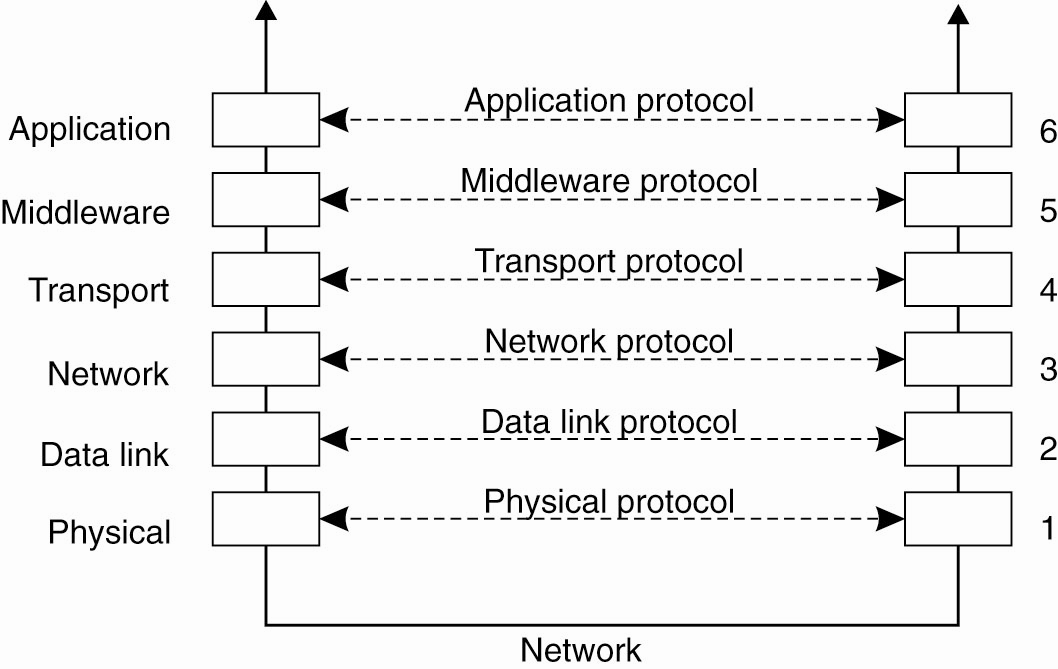
\includegraphics[scale=0.5]{img/osimid.png}
\caption{Modello OSI-Middleware}\label{img:osimid}
\end{figure}
\subsubsection{Tipi di comunicazione}
Esistono diverse alternative nella comunicazione che il middleware mette a disposizione delle applicazioni; partiamo dall'esempio mostrato in \figurename\,\ref{img:midcomuni}. In questo caso possiamo pensare che ogni \emph{host} esegua uno \emph{user agent} ovvero un processo che esegue le operazioni di comunicazione tra i vari sistemi.\\
\begin{figure}
\centering
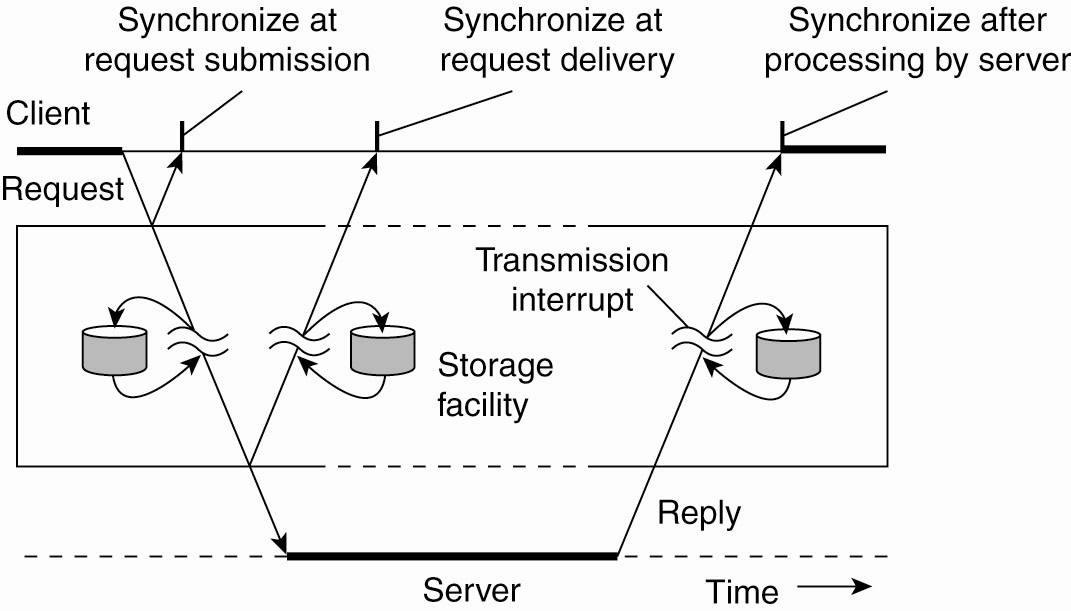
\includegraphics[scale=0.5]{img/midcomuni.png}
\caption{Esempio di tipi di comunicazione}\label{img:midcomuni}
\end{figure}
Prendiamo ora come esempio il caso di un invio di e-mail in questo caso i due \emph{user agent} saranno rispettivamente il sistema che invia e quello che riceve le e-mail. L'agente dal lato del mittente passa la mail al sistema per la consegna delle mail nella convinzione che tale sistema consegni la mail, l'agente dal lato del destinatario a sua volta si connette al sistema per sapere se è giunta qualche nuova mail in caso affermativo la mail viene trasferita dal sistema allo user agent del destinatario.\\
Questo tipo di meccanismo è detto \textbf{comunicazione persistente} in quanto il messaggio viene memorizzato dal middleware per tutto il tempo necessario affinché la consegna non vada a buon fine durante questo periodo non è necessario che i due elementi siano in esecuzione contemporaneamente. Nel caso di \textbf{comunicazione transiente} invece, il sistema memorizza i messaggi scambiati solo finché sia il mittente che il destinatario sono in esecuzione.\\
Oltre che persistente o transiente una comunicazione può essere asincrona o sincrona. Si parla di comunicazione \textbf{asincrona} quando il mittente continua la sua elaborazione subito dopo l'invio del messaggio. Nel caso di comunicazione \textbf{sincrona}, invece, il mittente è bloccato fino a quando la sua richiesta non viene accettata. Ciò può avvenire fino a quando il middleware non comunica la presa in consegna della richiesta, oppure quando la richiesta non viene consegnata al destinatario l'ultima possibilità è che il mittente resta bloccato fino alla fine dell'elaborazione da parte del destinatario e invio di una risposta all'elaborazione.\\
Esistono molti tipi in cui combinazione persistente, transiente, sincrona e asincrona possono essere combinati ma le più diffuse sono la persistenza e la sincronizzazione, la transiente con la sincronizzazione alla fine dell'elaborazione.\\
Dobbiamo distinguere, infine tra comunicazione discreta e a \emph{stream}.
\subsection{Chiamate a procedure remote}
Molti sistemi si basano sullo scambio di messaggi esplicito tra processi, questo scambio avviene tramite l'utilizzo delle procedure \texttt{send} e \texttt{recive} che però non nascondono del tutto la comunicazione. Una nuova tecnica fu introdotta nel 1984 quando si pensò di permettere ai programmi di richiamare procedure situate su altre macchine. Quando un processo sulla macchina $A$ richiama una procedura sulla macchina $B$ il processo chiamante viene sospeso e ha luogo l'elaborazione sulla macchina $B$. Le informazioni sono passate dal chiamante al chiamato tramite i parametri e ritornano indietro come risultato della procedura. Questo tipo di meccanismo è conosciuto come \textbf{chiamata a procedura remota } o \textbf{RPC} (\emph{remote procedure call}).\\
Sebbene l'idea di base risulti molto semplice i problemi relativi sono molti, primo fra tutti visto che chiamante e chiamata risiedono su due macchine diverse lo spazio degli indirizzi è completamente diverso, inoltre, il passaggio di parametri e dei risultati non è così semplice in quanto le macchine potrebbero avere rappresentazione dei dati differenti.
\subsubsection{Operazioni di base sulle RPC}
Iniziamo a vedere come funzionano realmente le RPC partendo dall'analisi di una chiamata a procedura locale per poi analizzare le chiamate remote.
\paragraph{Chiamate a procedura locali}
Per capire come lavorano le RPC è necessario capire comprendere come lavorano le chiamate a procedura convenzionali, ovvero su una singola macchina.
consideriamo una chiamate in C tipo:
\begin{center}
\texttt{count = read(fd, buf, nbytes)}
\end{center}
dove \emph{fd} è un intero che indica un file, \emph{buf} è un array di caratteri e \emph{nbytes} è il numero intero di byte da leggere ed immagazzinare in \emph{buf}.Se la chiamata è stata eseguita dal \emph{main} allora lo \emph{stack} della chiamata sarà quello mostrato in \figurename\,\ref{img:localstack}. Come vediamo nella figura (b) il chiamante inserisce (\emph{push}) i parametri nello stack in ordine inverso. Alla fine dell'esecuzione della procedura il valore di ritorno è posizionato in un registro vengono rimossi i parametri e viene restituito il controllo al chiamante.\\
\begin{figure}
\centering
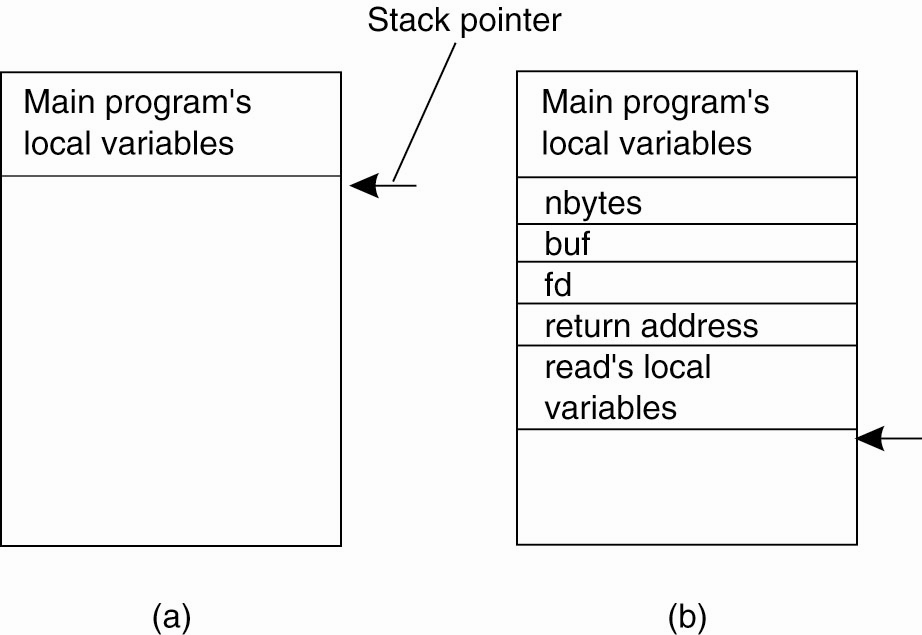
\includegraphics[scale=0.5]{img/localstack.png}
\caption{Stack prima e dopo la chiamata di una procedura}\label{img:localstack}
\end{figure}
Notiamo ora che in C i parametri possono essere passati per \textbf{valore} come \emph{fd} e \emph{nbytes} per i quali il valore viene copiato nello stack o per \textbf{referenza} come nel caso di \emph{buf} il quale è un puntatore ad un array di char; in questo caso nello stack della chiamata non vi è il valore dell'array ma semplicemente un indirizzo che indica dove l'array è situato. Nel caso in cui la procedura modifichi i valori contenuti nell'array tali cambiamenti saranno effettivi anche all'uscita dalla procedura.\\
Esiste un terzo meccanismo di passaggio dei parametri anche se non è usato in C ed è quello per \textbf{copia/ripristino}, questo passaggio consiste nel copiare il valore della variabile nello stack come nel caso di passaggio per valore, e quindi ricopiarla al termine della chiamata sovrascrivendo il valore originale. 
\paragraph{Client e server stub}
L'idea di base delle RPC è quella di rendere le chiamate a procedura remote il più simile possibile ad una chiamata locale. Vogliamo che le RPC siano trasparenti alla distribuzione. Per ottenere tale trasparenza quando il linker assembla il codice al posto di mettere la versione di sistema della procedura, nel nostro caso la \texttt{read}, esso la sostituisce con una versione chiamata \textbf{client stub}. Come quella originale anche questa versione viene richiamata usando la sequenza di \figurename\,\ref{img:localstack}, anche questa esegue una chiamata di sistema, ma a differenza di quella tradizionale questa chiamata impacchetta i dati in un messaggio e ne richiede l'invio al server tramite una \texttt{send}. Dopo l'invio il \emph{client stub} richiama la procedura \texttt{receive} e si blocca in attesa della risposta come mostrato in \figurename\,\ref{img:stub}.
\begin{figure}
\centering
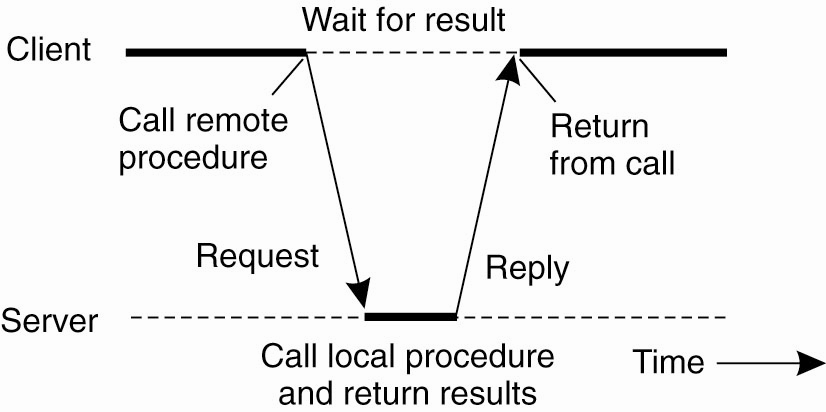
\includegraphics[scale=0.55]{img/stub.png}
\caption{Esempio di chiamata a procedura remota}\label{img:stub}
\end{figure}
Quando il messaggio raggiunge il server esso lo passa al \textbf{server sub}, l'equivalente lato server del \emph{client stub}, questo pezzo di codice trasforma la RPC in una chiamata a procedura locale. Il server esegue il proprio lavoro e restituisce il risultato al chiamante. Quando il \emph{server stub} riprende il controllo impacchetta il risultato in un messaggio e richiama la \texttt{send} per inviare la risposta al client e si rimette in attesa dell'arrivo di una nuova richiesta con la \texttt{receive}. Quando il messaggio di risposta arriva alla macchina client il sistema operativo lo indirizza al \emph{client stub} che lo spacchetta, copia i dati nel buffer e restituisce il controllo al processo client.\\
Quando il client riprende il controllo non ha idea di che cosa sia avvenuto e non ha idea se la chiamata è stata eseguita remotamente o in locale.
Ricapitolando una chiamata a procedura remota segue i seguenti passi:
\begin{enumerate}
\item la procedura client richiama il \emph{client stub} nel modo normale;
\item il \emph{client stub} costruisce un messaggio e richiama il sistema operativo locale;
\item il SO del client invia il messaggio al SO remoto;
\item il SO remoto passa il messaggio al \emph{server stub};
\item il \emph{server stub} spacchetta i parametri e richiama il server;
\item il server esegue il lavoro e restituisce il risultato allo \emph{stub};
\item il \emph{server stub} lo impacchetta in un messaggio e richiama il su SO;
\item il SO del server invia il messaggio al SO del client;
\item il SO del client passa il messaggio al \emph{client stub};
\item lo \emph{stub} spacchetta il risultato e lo restituisce al client.
\begin{figure}
\centering
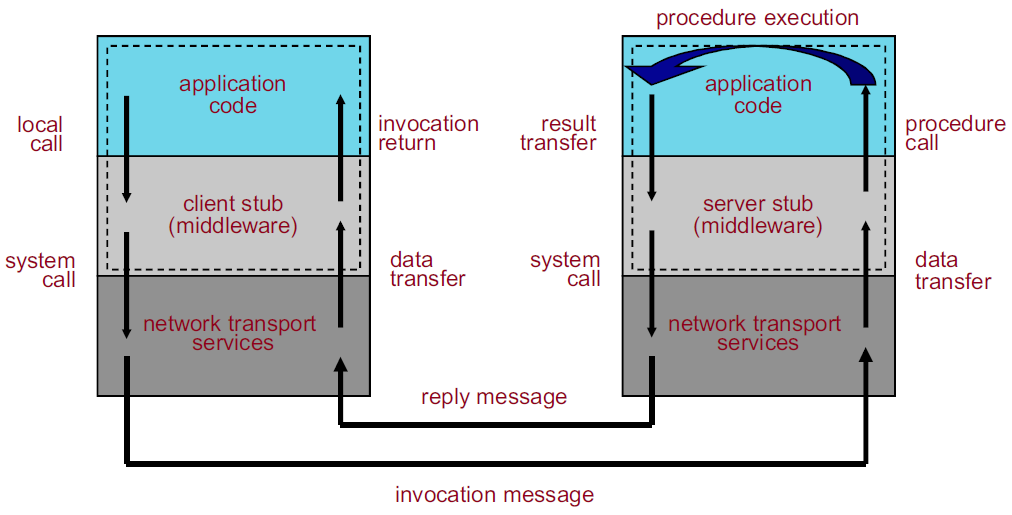
\includegraphics[scale=0.5]{img/execution.png}
\caption{Esecuzione di una chiamata a procedura a procedura remota}\label{img:executionrpc}
\end{figure}
\end{enumerate}
\subsubsection{Passaggio di parametri}
La funzione del client stub è quella di prendere i propri parametri di impacchettarli e di inviarli al server stub. Il problema è che questa operazione pur sembrando molto semplice in realtà non lo è.
\paragraph{Passaggio di parametri per valore}